\section{Causal architecture}

Let G denote measured constitutional variables; B(t), perinatal endocrine and physiological signals; M(t), microbial strains and functions; I(t), immune/metabolic conditions; A(t), early contact and affiliative regulation; C(t), molecular channel and synapse state; N(t), network state; R(t), regulatory phenotype; and E(t), the experienced environment. U terms represent unmeasured causes. A compact structural skeleton is:

\begin{align}
P_0 &= F(G,B_0,M_0,I_0,A_0,U_P),\\
C_{t+1} &= f_C(C_t,P_0,N_t,\nonumber\\
&\qquad I_t,E_t,U_C),\\
N_{t+1} &= f_N(N_t,C_t,E_t,A_t,U_N),\\
R_{t+1} &= f_R(R_t,N_t,\nonumber\\
&\qquad \mathrm{body}_t,E_t,U_R),\\
E_{t+1} &= f_E(E_t,R_t,\nonumber\\
&\qquad \mathrm{action}_t,\mathrm{institutions}_t,U_E).
\end{align}

These are proposed functional dependencies, not fitted laws. C must distinguish channel expression, surface localization, \ensuremath{\alpha_2\delta} isoform and cleavage, synaptic density, and measured release. N cannot be inferred from a peripheral biomarker alone. G is a vector; RCCX-specific measurements are one optional subset rather than the definition of constitution.

The unrolled graph is acyclic: R(t) \ensuremath{\rightarrow} E(t+1) \ensuremath{\rightarrow} N(t+2) \ensuremath{\rightarrow} R(t+3). A feedback arrow in the interactive master map summarizes this temporal sequence. It must not be interpreted as simultaneous reciprocal causation identified from cross-sectional correlations.

The core hinge hypothesis H1 states that a defined early perturbation changes a specified C component and that this change mediates a later N outcome. The parallel-path hypothesis H2 permits microbial or endocrine effects on N without C mediation. H3 concerns R \ensuremath{\times} E effects on performance and can survive rejection of H1. These nested alternatives make failure informative.


\begin{figure*}[t]
\centering
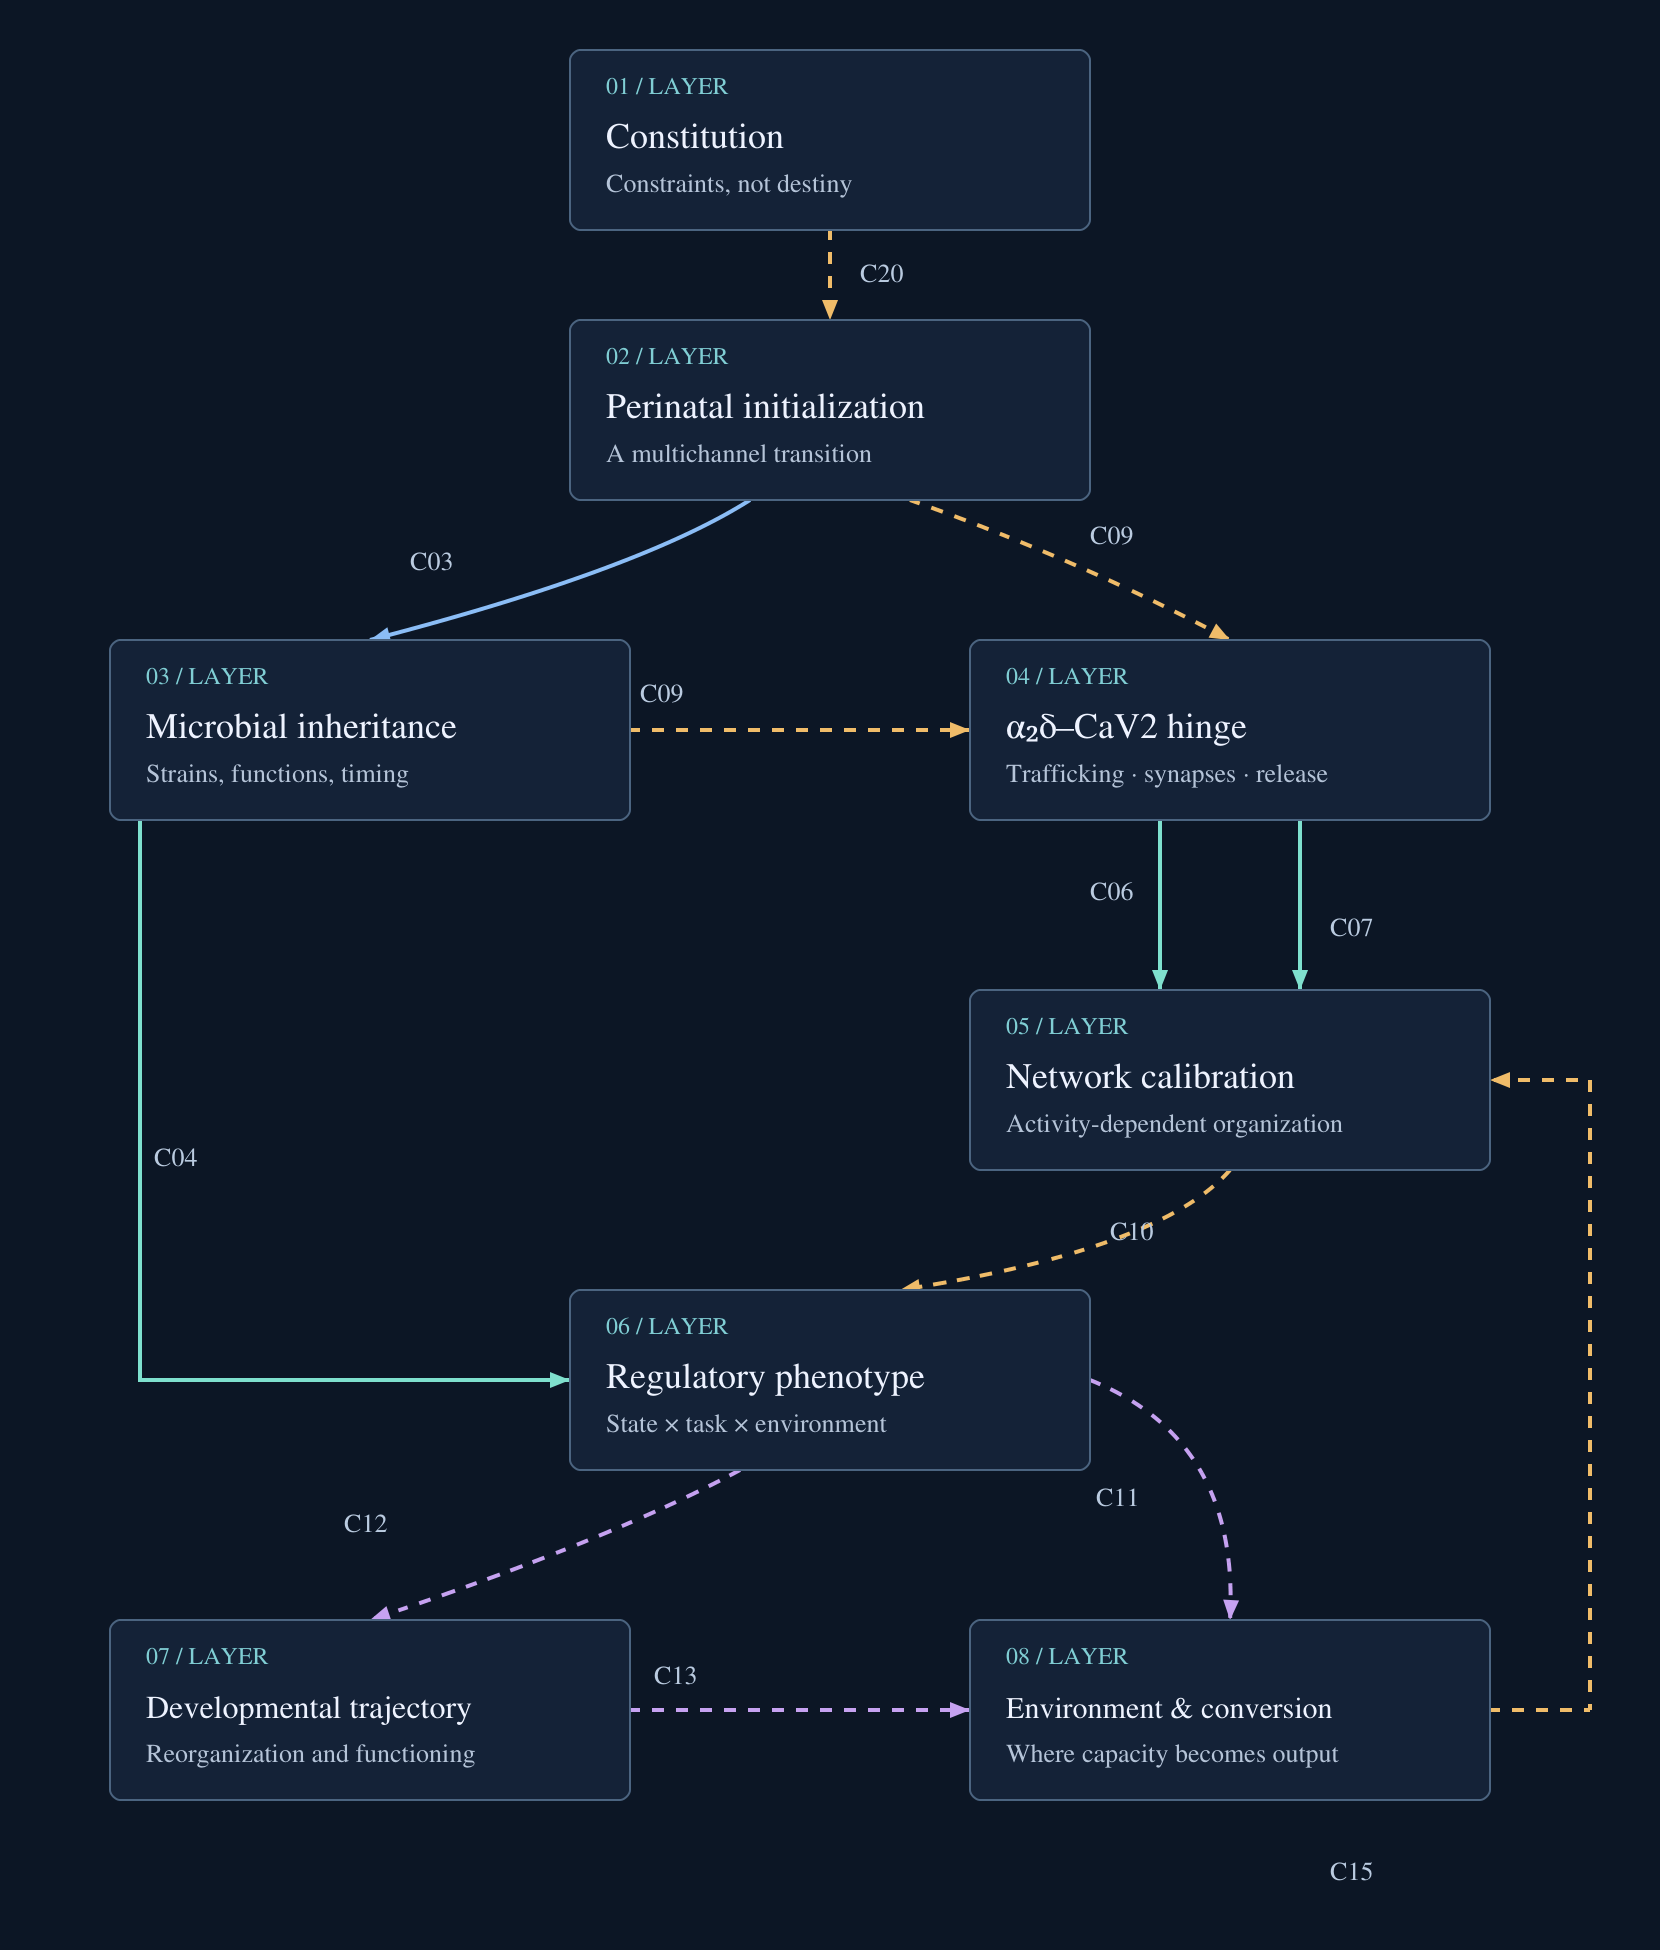
\includegraphics[height=5.6in,keepaspectratio]{../../assets/master-map.png}
\caption{Evidence-graded master field. Solid links concern bounded evidence; dashed links mark proposed bridges or horizon claims. Connection IDs resolve to the claim ledger. Feedback is indexed across time.}
\label{fig:master}
\end{figure*}
